%% 2018 CUMCM A 高温作业专用服装设计
%% 正文按 reasoning-preflight.json 已批准的三条路线扩写。
%% 数值全部取自 results/run-report.json 与 results/conclusions.json，由
%% solver/simulator.py 的同一次运行产生；未运行的量不写入正文。
\documentclass[withoutpreface,bwprint]{cumcmthesis}

\usepackage{amsmath}
\usepackage{booktabs}
\usepackage{graphicx}
\usepackage{siunitx}

\title{高温作业专用服装的多层瞬态传热建模与厚度设计}

\begin{document}

\begin{abstract}
假人皮肤外侧的实测温度在 \SI{5400}{s} 内由 \SI{37.00}{\celsius} 升到
\SI{48.08}{\celsius}，末十分钟波动为零，而环境温度是 \SI{75}{\celsius}。平台明显低于环境，
说明皮肤侧一直在把热量带走；附件 1 的密度使空气层扩散系数达到
\SI{2.361e-5}{m^2/s}，比其余三层高两个量级。这两件事决定了本文的模型形态：四层介质内的
一维瞬态热传导，界面处温度与热流同时连续，皮肤侧用一个散热系数代表血流带走的热量，
时间推进不能交给显式稳定域。

离散采用格心有限体积，界面导度取两侧半格热阻的调和平均，使热流连续成为离散格式的
精确性质而非近似；时间方向用后向 Euler。全模型只有散热系数一个自由参数。它由两条互相
独立的路线定出：仅用平台值的闭式解给 \SI{8.6124}{W/(m^2.K)}，对 5401 个实测点做最小二乘给
\SI{8.7739}{W/(m^2.K)}，相差 \SI{1.88}{\percent}。瞬态终点与解析稳态解相差 \SI{1e-10}{\celsius}，
格数由 10 加密到 80、步长由 \SI{4}{s} 缩到 \SI{1}{s} 时终点最大偏差 \SI{2.7e-9}{\celsius}，
全程残差均方根 \SI{0.4517}{\celsius}，末三十分钟 \SI{0.1453}{\celsius}。

问题二与问题三冻结上述仿真器与散热系数，只新开放厚度。题面的两条要求含时间，
必须写成逐时刻上限与越阈累计时长两个瞬态判据，而不是一个稳态温度。实测确认皮肤温度峰值
随第 II 层厚度单调不增，因此最小可行厚度用一维二分求得：\SI{65}{\celsius}、六十分钟、
第 IV 层 \SI{5.5}{mm} 时为 \SI{18.16}{mm}，此时峰值仅 \SI{44.045}{\celsius}，紧的是五分钟预算
而不是 \SI{47}{\celsius} 上限，皮肤温度首次越过 \SI{44}{\celsius} 的时刻恰在第 \SI{55}{min}。
问题三两个目标方向相反且题面未给交换率，故不作相减标量化：第 IV 层薄于 \SI{3.6}{mm} 时
第 II 层取遍整个允许区间都不可行，可行性边界约在 \SI{3.8}{mm}；前沿从
$(d_4,d_2)=(3.8,24.99)$ 延伸到 $(6.4,21.19)$，总厚最小点为 \SI{21.188}{mm} 与 \SI{6.4}{mm}。

最优点的平台温度只比阈值高 \SI{0.14}{\celsius}，而第 \SI{55}{min} 处曲线斜率仅
\SI{0.0112}{\celsius\per\minute}。散热系数变动 \SI{2}{\percent}（即标定自身精度）就使最优厚度
在 \SI{17.04}{mm} 与 \SI{19.19}{mm} 之间移动，变动 \SI{20}{\percent} 时可行域从整体不可行跳到
下界即可行。该约束在本题是病态的，因此本文交付区间与机理，不给三位有效数字的设计值。
\end{abstract}

\keywords{多层瞬态传热\quad 有限体积\quad 界面热流连续\quad 越阈时长约束\quad 可辨识区间}

\section{问题重述}
\label{mcm-body-start}

高温作业服由三层织物构成，自外向内记为第 I、II、III 层，第 III 层与皮肤之间的空隙记为
第 IV 层。把体温维持在 \SI{37}{\celsius} 的假人放入高温环境，测量其皮肤外侧温度，据此为
服装选厚度。附件 1 给出四层的密度、比热、热传导率与厚度：第 I 层 \SI{0.6}{mm}、第 III 层
\SI{3.6}{mm} 固定，第 II 层允许 \SI{0.6}{mm} 到 \SI{25}{mm}，第 IV 层允许 \SI{0.6}{mm} 到
\SI{6.4}{mm}。附件 2 是 \SI{75}{\celsius} 环境下、第 II 层 \SI{6}{mm}、第 IV 层 \SI{5}{mm}、
九十分钟工作时长这一组条件的皮肤外侧温度记录，逐秒共 5401 点。

三个问题依次是：在附件 2 对应的条件下算出温度分布并输出到 Excel；在 \SI{65}{\celsius}、
第 IV 层 \SI{5.5}{mm} 时定第 II 层最优厚度，使六十分钟内皮肤外侧温度不超过
\SI{47}{\celsius}，且超过 \SI{44}{\celsius} 的时间不超过五分钟；在 \SI{80}{\celsius} 时同时定
第 II、IV 层最优厚度，三十分钟内满足同一组温度要求。降低研发成本、缩短研发周期是选厚度的
背景动机，它在数学上表现为“在满足温度要求的前提下第 II 层越薄越好”。

需要说明来源边界。本文使用的题面文字取自一份参考论文的问题重述，不是官方题面原件；
官方材料只有附件 1 与附件 2 两张表。所有数值结论都只依赖这两张表和本文自己的计算，
不依赖那份参考论文的任何结果。

\section{问题分析}

三问不是三个独立任务。问题一有实测曲线可比对，是唯一能确定未知参数的一问；问题二、三没有
新的实测数据，只更换环境温度、时长和待定厚度。所以问题一的产物必须是一个能被后两问反复
调用的计算核心，而不是一张图。后两问冻结这个核心与它标定出的参数，各自只新开放厚度。
若某一问改用另一套无需时间的代数式来定厚度，它就不再共享问题一的时间维，题面里的
“六十分钟”“三十分钟”“不超过五分钟”都会失去表达位置。

先看附件 2 能读出什么。温度从 \SI{37.00}{\celsius} 起，在 \SI{1261}{s}（第 \SI{21.0}{min}）
之后每分钟变化已小于 \SI{0.01}{\celsius}，末十分钟稳定在 \SI{48.08}{\celsius}、波动为零。
平台值远低于环境的 \SI{75}{\celsius}，这排除了皮肤侧绝热：若皮肤侧不导出热量，整个系统最终
会趋于环境温度。因此皮肤侧必须写成一个把热量送往体核的边界，其强度是全模型唯一待定量。

再看附件 1 的物性会带来什么数值后果。第 $i$ 层的热扩散系数
$a_i=\lambda_i/(\rho_i c_i)$，逐层计算后，第 I 至 III 层的扩散
系数在 \SI{2e-7}{m^2/s} 量级，而第 IV 层因密度只有 \SI{1.18}{kg/m^3} 而达到
\SI{2.361e-5}{m^2/s}。显式格式的稳定条件 $r=a\tau/h^2\le 1/2$ 会被这一层控制，把时间步长压到
远小于一秒。这一点直接决定时间推进方式，而不是事后调参的问题。这里还有一个容易被掩盖的
陷阱：若把导热系数 $\lambda$ 误当作扩散系数代入同一显式格式，步长比反而落在稳定域内，
程序照样输出光滑曲面。数值稳定并不证明系数正确，因此本文把逐层 $a$ 与附件 1 预置列逐位对账，
作为一道单独的检查。

两问的约束读法也需要先定。“六十分钟内不超过 \SI{47}{\celsius}”是逐时刻上限，
“超过 \SI{44}{\celsius} 的时间不超过五分钟”是越阈累计时长。皮肤温度单调上升并趋于平台，
所以第二条等价于“不得在第 \SI{55}{min} 之前越过 \SI{44}{\celsius}”。这两个量都需要完整的
温度历程才能计算，稳态温度给不出其中任何一个。

\section{模型假设}

假设只保留会改变方程或约束的四条，每条都注明它改动了哪一部分数学对象。

第一，传热沿垂直于皮肤的方向进行，四层介质在该方向上均质。这把三维问题降为一维，
使每层只需一个厚度、一个扩散系数。

第二，各层界面处温度与热流同时连续。这给出层间耦合条件，是有限体积中界面导度取调和平均的
依据；若只要求温度连续，界面处的能量就不守恒。

第三，第 I 层外表面温度等于环境温度。这把外侧边界定为 Dirichlet 型。该假设在升温初段偏强，
本文在检验一节用残差结构如实报告它的代价，不作修正。

第四，皮肤侧向体核的散热强度与皮肤外侧温度和体核温度之差成正比，体核温度维持
\SI{37}{\celsius}。这把体内的血流散热压缩成一个系数，使全模型只剩一个待定参数；代价是该系数
只能由 \SI{75}{\celsius} 的那次实验定出，跨环境温度的可迁移性没有证据，本文在灵敏度一节
单独处理。

不考虑湿传递与辐射。这不是为了简化方程，而是因为附件只给了干态热物性，没有任何可用于
标定湿传递或辐射的量；把它们写进方程会引入无法确定的参数。

\section{符号说明}

\begin{table}[htbp]
  \centering
  \caption{贯穿全文的符号}
  \label{tab:symbols}
  \begin{tabular}{cll}
    \toprule
    符号 & 含义 & 单位 \\
    \midrule
    $x$ & 自第 I 层外表面算起的深度 & \si{m} \\
    $T(x,t)$ & 深度 $x$、时刻 $t$ 的温度 & \si{\celsius} \\
    $\rho_i,\ c_i,\ \lambda_i$ & 第 $i$ 层的密度、比热、热传导率 & \si{kg/m^3},\ \si{J/(kg.K)},\ \si{W/(m.K)} \\
    $a_i=\lambda_i/(\rho_i c_i)$ & 第 $i$ 层的热扩散系数 & \si{m^2/s} \\
    $d_i$ & 第 $i$ 层厚度，$d_2$、$d_4$ 为决策变量 & \si{mm} \\
    $T_{\mathrm{env}}$ & 环境温度 & \si{\celsius} \\
    $T_{\mathrm{core}}$ & 体核温度，取 \num{37} & \si{\celsius} \\
    $h$ & 皮肤侧散热系数，全模型唯一待定参数 & \si{W/(m^2.K)} \\
    $\theta(t)$ & 皮肤外侧温度，即 $x=L$ 处的温度 & \si{\celsius} \\
    $q$ & 稳态下通过服装的热流密度 & \si{W/m^2} \\
    $R$ & 四层串联总热阻 & \si{m^2.K/W} \\
    $T_{\mathrm{w}}$ & 工作时长，问题二为 \num{3600}、问题三为 \num{1800} & \si{s} \\
    \bottomrule
  \end{tabular}
\end{table}

附件 1 给出的物性列在表~\ref{tab:props}。最后一列是按 $a_i=\lambda_i/(\rho_i c_i)$ 换算的
热扩散系数，与附件 1 自带的预置列逐位一致，本文以它作为方程系数。表中第 II、IV 层的厚度
是允许区间而非定值，这两个区间就是问题二、三的决策变量取值范围。

\begin{table}[htbp]
  \centering
  \caption{附件 1 的四层物性与换算所得热扩散系数}
  \label{tab:props}
  \begin{tabular}{cccccc}
  \toprule
    层 & $\rho$/\si{kg/m^3} & $c$/\si{J/(kg.K)} & $\lambda$/\si{W/(m.K)} & $d$/\si{mm} & $a$/\si{m^2/s} \\
  \midrule
    I & 300 & 1377 & 0.082 & 0.6 & \num{1.985e-07} \\
    II & 862 & 2100 & 0.37 & 0.6--25 & \num{2.044e-07} \\
    III & 74.2 & 1726 & 0.045 & 3.6 & \num{3.514e-07} \\
    IV & 1.18 & 1005 & 0.028 & 0.6--6.4 & \num{2.361e-05} \\
  \bottomrule
\end{tabular}

\end{table}

值得先注意第 IV 层。它是空气层，密度只有 \SI{1.18}{kg/m^3}，因此在四层中同时具有最大的
热阻和最快的扩散：热阻大意味着它决定能挡住多少热量，扩散快意味着它几乎不延迟热量到达皮肤。
这两个性质在后面三问里反复起作用。

\section{问题一模型建立与求解}
\label{mcm-q1-start}

\subsection{模型建立}

设四层总厚 $L=\sum_i d_i$。在每一层内部，能量守恒给出
\begin{equation}
  \rho_i c_i \frac{\partial T}{\partial t}
  = \frac{\partial}{\partial x}\!\left(\lambda_i \frac{\partial T}{\partial x}\right),
  \qquad x \in \text{第 } i \text{ 层}.
  \label{eq:pde}
\end{equation}
相邻层界面 $x_{i}$ 处同时要求
\begin{equation}
  T(x_i^-,t)=T(x_i^+,t), \qquad
  \lambda_i \left.\frac{\partial T}{\partial x}\right|_{x_i^-}
  = \lambda_{i+1} \left.\frac{\partial T}{\partial x}\right|_{x_i^+}.
  \label{eq:interface}
\end{equation}
外侧按假设三取 $T(0,t)=T_{\mathrm{env}}$。皮肤侧由前一节的平台观察定为
\begin{equation}
  -\lambda_4 \left.\frac{\partial T}{\partial x}\right|_{x=L}
  = h\,\bigl(T(L,t)-T_{\mathrm{core}}\bigr).
  \label{eq:robin}
\end{equation}
初始时刻全场取 \SI{37}{\celsius}，与附件 2 的 $t=0$ 读数一致。皮肤外侧温度
$\theta(t)=T(L,t)$ 即与附件 2 对应的观测量。

式~\eqref{eq:pde}--\eqref{eq:robin} 在稳态下退化为串联平板关系，可用于交叉校核：
\begin{equation}
  q=\frac{T_{\mathrm{env}}-T_{\mathrm{core}}}{R+1/h},
  \qquad R=\sum_{i=1}^{4}\frac{d_i}{\lambda_i},
  \qquad \theta_{\infty}=T_{\mathrm{core}}+\frac{q}{h}.
  \label{eq:steady}
\end{equation}
按附件 2 的条件，$R=\SI{0.282105}{m^2.K/W}$。表~\ref{tab:res} 把它拆到每一层，同时给出
稳态温降与扩散时间尺度 $d_i^2/a_i$。

\begin{table}[htbp]
  \centering
  \caption{附件 2 条件下的逐层热阻、稳态温降与扩散时间尺度}
  \label{tab:res}
  \begin{tabular}{cccccc}
  \toprule
    层 & $d$/\si{mm} & $d/\lambda$/\si{m^2.K/W} & 占总热阻/\si{\percent} & 稳态温降/\si{\celsius} & $d^2/a$/\si{s} \\
  \midrule
    I & 0.6 & 0.007317 & 2.6 & 0.698 & 1.8 \\
    II & 6.0 & 0.016216 & 5.7 & 1.547 & 176.1 \\
    III & 3.6 & 0.080000 & 28.4 & 7.634 & 36.9 \\
    IV & 5.0 & 0.178571 & 63.3 & 17.040 & 1.1 \\
  \midrule
    合计 & 15.2 & 0.282105 & 100.0 & 26.920 & --- \\
  \bottomrule
\end{tabular}

\end{table}

三件事从这张表读出来。第一，空气层占总热阻 \SI{63.3}{\percent}，单独承担
\SI{17.040}{\celsius} 温降，这解释了问题三中第 IV 层厚度为何能决定可行性。第二，
第 III 层热阻占 \SI{28.4}{\percent}，而第 II 层只占 \SI{5.7}{\percent}——第 II 层加厚
对隔热的边际贡献本来就小，这预示问题二的最优厚度会偏大。第三，四层的扩散时间尺度都在
\SI{200}{s} 以内，最长的第 II 层是 \SI{176.1}{s}；整叠的等效时间尺度取总厚与最小扩散
系数之比约为 \SI{1160}{s}，与附件 2 在第 \SI{21}{min} 进入准稳态相符。这个量级说明
三问的时间窗都长于系统的响应时间，但不等于可以用稳态代替瞬态——判据里的五分钟正好落在
响应尾段。

\subsection{求解方法与实现}

把区间 $[0,L]$ 按层划分为格心控制体，第 $i$ 层分 $n_i$ 格、格宽 $h_i=d_i/n_i$。格数按层厚
分配，并令最薄的一层不少于 8 格，使 \SI{0.6}{mm} 的第 I 层与每个界面都能被分辨；本文实际
使用的总格数在 253 到 2027 之间。

离散不从式~\eqref{eq:pde} 直接差分，而从控制体的能量平衡出发。对第 $j$ 格在
$[t^n,t^{n+1}]$ 内积分式~\eqref{eq:pde}，并把左右两个面上的热流记为 $q_{j-1/2}$、
$q_{j+1/2}$，得
\begin{equation}
  \rho_j c_j h_j \frac{T_j^{n+1}-T_j^{n}}{\tau}
  = q_{j-1/2}-q_{j+1/2},
  \qquad
  q_{j+1/2}=-K_{j+1/2}\bigl(T_{j+1}-T_j\bigr).
  \label{eq:fv}
\end{equation}
这样写的好处是：无论 $\lambda$ 在界面处如何跳变，进入一格的热量与离开相邻一格的热量
用的是同一个 $q_{j+1/2}$，能量在离散层面自动守恒，不需要额外的界面方程。

界面导度 $K_{j+1/2}$ 由两个半格串联的热阻定出。从格心 $j$ 到界面的热阻是
$h_j/(2\lambda_j)$，从界面到格心 $j+1$ 是 $h_{j+1}/(2\lambda_{j+1})$，串联相加再取倒数：
\begin{equation}
  K_{j+1/2}=\left(\frac{h_j}{2\lambda_j}+\frac{h_{j+1}}{2\lambda_{j+1}}\right)^{-1}.
  \label{eq:harmonic}
\end{equation}
这正是式~\eqref{eq:interface} 的离散对应。若改用算术平均
$\tfrac12(\lambda_j+\lambda_{j+1})$，在第 III 层与第 IV 层界面处
$\lambda$ 相差 \num{1.6} 倍，界面热流会被系统性高估；本题空气层与织物层的导热系数
相差一个量级，这一选择不是精度上的微调。

时间方向的选择由前一节的扩散系数量级决定。空气层的 $a=\SI{2.361e-5}{m^2/s}$ 使显式格式的
稳定步长远小于一秒，而实测数据的采样间隔恰是一秒。因此本文用后向 Euler，对格 $j$ 有
\begin{equation}
  \frac{C_j}{\tau}\bigl(T_j^{n+1}-T_j^{n}\bigr)
  = K_{j-1/2}\bigl(T_{j-1}^{n+1}-T_j^{n+1}\bigr)
  + K_{j+1/2}\bigl(T_{j+1}^{n+1}-T_j^{n+1}\bigr),
  \qquad C_j=\rho_j c_j h_j,
  \label{eq:implicit}
\end{equation}
两端按 Dirichlet 与式~\eqref{eq:robin} 的 Robin 形式并入对角。每一时间层是一个三对角系统，
按带状矩阵直接求解，无条件稳定，步长由需要的输出分辨率决定而不再由空气层决定。

把式~\eqref{eq:implicit} 写成矩阵形式便于说明两端如何并入。记
$\boldsymbol{T}^{n}=(T_1^n,\dots,T_N^n)^{\mathsf T}$，则
\begin{equation}
  \left(\mathrm{diag}\!\left(\frac{C_j}{\tau}\right)+\boldsymbol{A}\right)\boldsymbol{T}^{n+1}
  = \mathrm{diag}\!\left(\frac{C_j}{\tau}\right)\boldsymbol{T}^{n}+\boldsymbol{b},
  \label{eq:matrix}
\end{equation}
其中 $\boldsymbol{A}$ 是由各 $K_{j\pm1/2}$ 组成的三对角矩阵。外侧 Dirichlet 条件不引入
额外未知量：它以 $K_{1/2}=2\lambda_1/h_1$ 的形式加到 $\boldsymbol{A}$ 的首个对角元上，
同时把 $K_{1/2}T_{\mathrm{env}}$ 加进 $\boldsymbol{b}$ 的首项。皮肤侧的 Robin 条件同理，
只是导度取半格热阻与外部散热的串联
\begin{equation}
  K_{N+1/2}=\left(\frac{h_N}{2\lambda_4}+\frac{1}{h}\right)^{-1},
  \label{eq:robindisc}
\end{equation}
并把 $K_{N+1/2}T_{\mathrm{core}}$ 加进 $\boldsymbol{b}$ 的末项。$\boldsymbol{A}$ 的对角元
严格大于同行非对角元绝对值之和加边界导度，因此系数矩阵是不可约对角占优的，解存在且唯一，
数值上也不需要预处理。

皮肤外侧温度不是最后一格的格心值。它是 $x=L$ 处的面温，由该格心到面的半格热阻与外部散热
串联定出：
\begin{equation}
  \theta = \frac{\bigl(2\lambda_4/h_N\bigr)T_N + h\,T_{\mathrm{core}}}
                {2\lambda_4/h_N + h}.
  \label{eq:face}
\end{equation}
若直接用 $T_N$ 代替 $\theta$，在空气层格宽下会引入系统性偏差，这一点在与附件 2 对比时会被
残差直接暴露。

离散是否足够细需要当场验证，而不是留到检验一节。表~\ref{tab:grid} 给出 12 组网格与步长
组合下的终点温度。

\begin{table}[htbp]
  \centering
  \caption{网格与时间步长组合下的终点温度（附件 2 条件）}
  \label{tab:grid}
  \begin{tabular}{ccccc}
  \toprule
    最薄层格数 & $\tau$/\si{s} & 总格数 & 终点温度/\si{\celsius} & 与最细网格之差/\si{\celsius} \\
  \midrule
    10 & 4 & 253 & 47.934716683 & \num{1.6e-09} \\
    10 & 2 & 253 & 47.934716683 & \num{1.6e-09} \\
    10 & 1 & 253 & 47.934716683 & \num{1.6e-09} \\
    20 & 4 & 507 & 47.934716683 & \num{1.6e-09} \\
    20 & 2 & 507 & 47.934716683 & \num{1.5e-09} \\
    20 & 1 & 507 & 47.934716683 & \num{1.6e-09} \\
    40 & 4 & 1013 & 47.934716683 & \num{1.5e-09} \\
    40 & 2 & 1013 & 47.934716682 & \num{2.3e-09} \\
    40 & 1 & 1013 & 47.934716683 & \num{1.5e-09} \\
    80 & 4 & 2027 & 47.934716681 & \num{2.7e-09} \\
    80 & 2 & 2027 & 47.934716682 & \num{1.7e-09} \\
    80 & 1 & 2027 & 47.934716684 & \num{0} \\
  \bottomrule
\end{tabular}

\end{table}

最薄层格数由 10 加到 80、步长由 \SI{4}{s} 缩到 \SI{1}{s}，总格数从 253 变到 2027，
终点温度的相互偏差始终在 \SI{3e-9}{\celsius} 以内。偏差这么小有具体原因：
式~\eqref{eq:harmonic} 的调和平均使界面热流在离散层面精确守恒，界面不再是误差来源；
后向 Euler 又无条件稳定，步长只影响时间分辨率而不影响终态。因此后文一律用最薄层
20 格、步长 \SI{2}{s} 做厚度搜索，用 \SI{1}{s} 做与附件 2 的逐秒对比。

\subsection{标定与本问结果}

$h$ 由两条互不依赖的路线定出。第一条只用平台值：把附件 2 的末值 \SI{48.08}{\celsius} 代入
式~\eqref{eq:steady} 反解，得 $h=\SI{8.6124}{W/(m^2.K)}$；它完全不看瞬态形状。第二条对全部
5401 个实测点做最小二乘，得 $h=\SI{8.7739}{W/(m^2.K)}$，残差均方根
\SI{0.4517}{\celsius}。两者相差 \SI{1.88}{\percent}。之所以要做两条，是因为单靠最小二乘无法
区分“拟合得好”与“结构对”——若边界形式选错，最小二乘仍会找到一个使曲线尽量贴合的系数，
而闭式路线只受平台约束。两条给出接近的值，说明式~\eqref{eq:robin} 的结构没有被拟合掩盖。
下文一律使用最小二乘值。

\begin{table}[htbp]
  \centering
  \caption{散热系数的两条标定路线}
  \label{tab:cal}
  \begin{tabular}{lccl}
  \toprule
    标定路线 & 使用的数据 & $h$/\si{W/(m^2.K)} & 说明 \\
  \midrule
    闭式反解 & 仅平台值 \SI{48.08}{\celsius} & 8.6124 & 不看瞬态形状 \\
    最小二乘 & 全部 5401 点 & 8.7739 & 残差均方根 \SI{0.4517}{\celsius} \\
  \midrule
    相对差 & --- & \SI{1.88}{\percent} & 结构未被拟合掩盖 \\
  \bottomrule
\end{tabular}

\end{table}

表~\ref{tab:cal} 把两条路线并列。需要强调它们的独立性：闭式路线只用一个数（末值
\SI{48.08}{\celsius}），把式~\eqref{eq:steady} 反解，完全不涉及升温过程；最小二乘路线
用全部 5401 个点，但不单独约束末值。若边界形式选错——例如把皮肤侧写成绝热或写成第二类
边界——最小二乘仍会找出一个使曲线尽量贴合的系数，而闭式路线给出的值会与它明显分离。
两者相差 \SI{1.88}{\percent} 才使“结构选对了”这一判断有依据。

在附件 2 的条件下推进 \SI{5400}{s}，模型给出的皮肤外侧终点温度为
\SI{47.9347}{\celsius}，实测末值 \SI{48.08}{\celsius}。稳态界面温度依次为
\num{74.30}、\num{72.76}、\num{65.12}、\SI{47.93}{\celsius}，与式~\eqref{eq:steady} 的
逐层温降一致。温度分布 $T(x,t)$ 按逐秒、逐格导出为 Excel，随支撑材料提交，
其中横向为深度、纵向为时间。

图~\ref{fig:q1fit} 上半给出模型与附件 2 的逐秒对比，下半是残差。两条曲线在
第 \SI{20}{min} 以后基本重合，残差在此后落在 $\pm\SI{0.2}{\celsius}$ 之内；
偏差集中在最初十分钟，模型升温快于实测。这与假设三直接对应，
下一节把它量化为分段残差。

\begin{figure}[htbp]
  \centering
  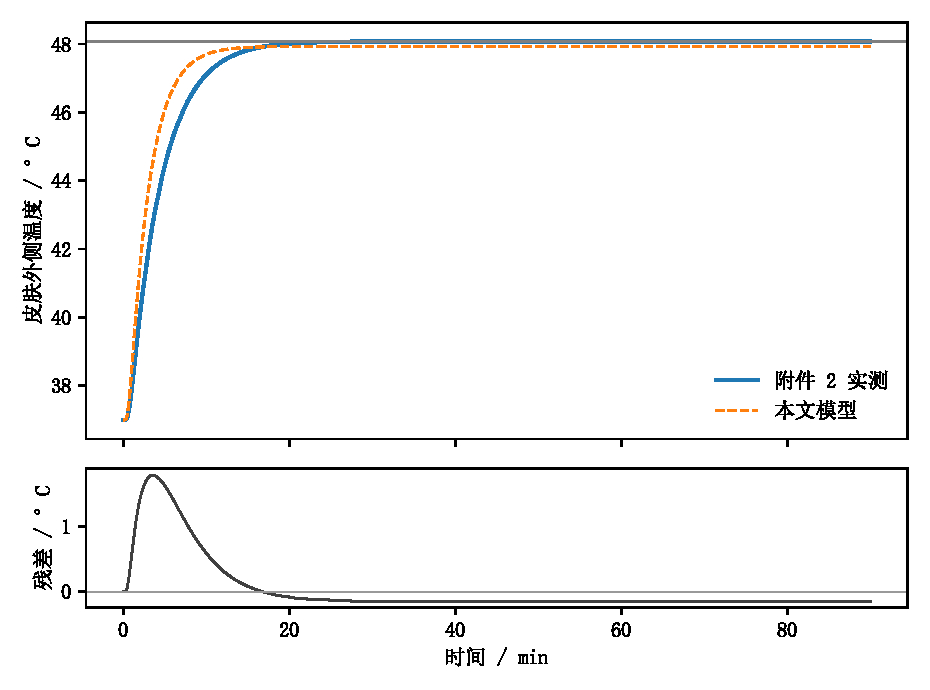
\includegraphics[width=0.86\textwidth]{figures/fig-q1-fit.pdf}
  \caption{皮肤外侧温度：模型与附件 2 实测对比及残差}
  \label{fig:q1fit}
\end{figure}

表~\ref{tab:hist} 取几个时刻列出模型给出的皮肤外侧温度，图~\ref{fig:q1prof} 则给出同一次
运行的层内温度剖面。剖面图上竖线是层界。第 \SI{1}{min} 时热量还集中在前两层，
第 \SI{5}{min} 时第 III 层开始升温，第 \SI{21}{min} 与第 \SI{90}{min} 的两条曲线几乎重合，
说明系统此时已进入准稳态。剖面在空气层内的陡降对应表~\ref{tab:res} 里那
\SI{17.040}{\celsius}，这是全叠温降的主要来源。

\begin{table}[htbp]
  \centering
  \caption{模型给出的皮肤外侧温度演化（附件 2 条件）}
  \label{tab:hist}
  \begin{tabular}{cc}
  \toprule
    时刻/\si{min} & 模型皮肤外侧温度/\si{\celsius} \\
  \midrule
    1 & 38.4459 \\
    5 & 46.0809 \\
    10 & 47.7017 \\
    21 & 47.9323 \\
    45 & 47.9347 \\
    90 & 47.9347 \\
  \bottomrule
\end{tabular}

\end{table}

\begin{figure}[htbp]
  \centering
  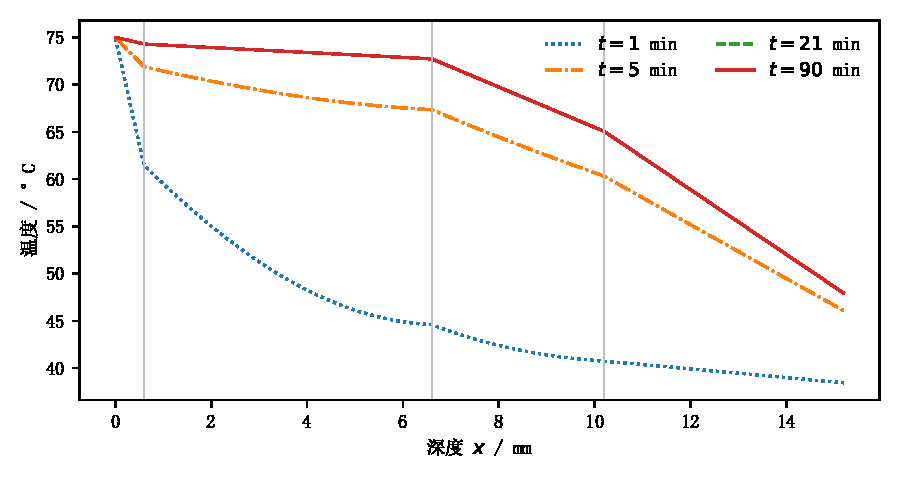
\includegraphics[width=0.84\textwidth]{figures/fig-q1-profile.pdf}
  \caption{四层内的温度剖面随时间演化，竖线为层界}
  \label{fig:q1prof}
\end{figure}

本问还剩一处边界要交代。式~\eqref{eq:robin} 的散热系数只由 \SI{75}{\celsius} 这一次实验
定出，本问不涉及外推，因此它在本问是标定量而非假设；但问题二、三要在 \SI{65}{\celsius} 与
\SI{80}{\celsius} 下沿用同一个值，那时它就变成一个未经验证的外推。另外假设三把第 I 层外
表面温度直接取为环境温度，这在升温初段偏强，其代价由下节的分段残差给出，本文不作修正，
也因此不宣称模型在最初十分钟内可用。

\section{问题二模型建立与求解}
\label{mcm-q1-end}
\label{mcm-q2-start}

\subsection{约束的瞬态表达}

本问冻结问题一的仿真器与 $h=\SI{8.7739}{W/(m^2.K)}$，环境温度改为 \SI{65}{\celsius}，
第 IV 层固定 \SI{5.5}{mm}，唯一新开放的量是 $d_2$，其允许范围由附件 1 给定为
$[\num{0.6},\num{25}]\,\si{mm}$。题面的两条要求写成
\begin{equation}
  \max_{0\le t\le T_{\mathrm{w}}}\theta(t)\le \SI{47}{\celsius},
  \qquad
  \bigl|\{t\in[0,T_{\mathrm{w}}]:\theta(t)>\SI{44}{\celsius}\}\bigr| \le \SI{300}{s},
  \label{eq:crit}
\end{equation}
其中 $T_{\mathrm{w}}=\SI{3600}{s}$。第二式是越阈累计时长，需要完整历程；由于 $\theta$ 单调
上升趋于平台，它等价于“首次越过 \SI{44}{\celsius} 不早于第 \SI{55}{min}”。

记 $\theta(t;d_2)$ 为由式~\eqref{eq:pde}--\eqref{eq:robin} 在给定 $d_2$ 下解出的皮肤外侧温度，
本问的优化问题即
\begin{equation}
  \min_{d_2}\ d_2
  \quad \text{s.t.}\quad
  \max_{0\le t\le T_{\mathrm{w}}}\theta(t;d_2)\le 47,\quad
  \int_{0}^{T_{\mathrm{w}}}\mathbf{1}\{\theta(t;d_2)>44\}\,\mathrm{d}t \le 300,\quad
  0.6\le d_2\le 25 .
  \label{eq:opt2}
\end{equation}
两条约束都以 $\theta(\cdot;d_2)$ 为中介依赖决策变量，没有闭式形式；这是本问必须调用
问题一仿真器而不能另列代数式的直接原因。目标函数取 $d_2$ 本身，对应题面“降低研发成本”
在本问的唯一可量化含义：其余三层厚度均已固定，成本只随第 II 层用料变化。

这里有一条被排除的路线值得写明，因为它看起来更省事。若只写稳态串联式并令皮肤温度等于
\SI{47}{\celsius}，得到的是四个界面方程对 $\theta_2,\theta_3,\theta_4,q,d_2$ 五个未知量，
少一个条件。实际扫描 $d_2=\num{0.6},\num{2.0},\num{5.5},\num{10.0},\SI{25.0}{mm}$ 时，
每个厚度都能配出一组自洽的界面温度，热流依次为 \num{63.08}、\num{62.25}、\num{60.28}、
\num{57.92}、\SI{51.24}{W/m^2}。也就是说该方程组不约束 $d_2$；若再以“$d_2$ 最小”为目标，
最优解只会落到下界 \SI{0.6}{mm}。更根本的是稳态温度是常数，一旦它高于 \SI{44}{\celsius}，
越阈时长就等于剩余全部工作时间，式~\eqref{eq:crit} 的第二条退化成“平台温度不超过
\SI{44}{\celsius}”，比题目要求严得多。故本问不使用稳态式定厚度，只把它留作问题一的校核。

\subsection{搜索层与求解}

在给出搜索方法之前先确认可行集的形状。固定其余条件，令 $d_2$ 取遍允许区间，
皮肤温度峰值的变化见表~\ref{tab:mono}。

\begin{table}[htbp]
  \centering
  \caption{第 II 层厚度对皮肤温度峰值与越阈时长的影响（\SI{65}{\celsius}，六十分钟，$d_4=\SI{5.5}{mm}$）}
  \label{tab:mono}
  \begin{tabular}{cccccccc}
    \toprule
    $d_2$/\si{mm} & 0.600 & 3.000 & 6.000 & 10.000 & 14.000 & 18.161 & 25.000 \\
    \midrule
    峰值/\si{\celsius} & 44.991 & 44.864 & 44.710 & 44.513 & 44.318 & 44.045 & 43.240 \\
    $>\SI{44}{\celsius}$ 时长/\si{s} & 3548 & 3442 & 3210 & 2698 & 1854 & 300 & 0 \\
    \bottomrule
  \end{tabular}
\end{table}

峰值随厚度单调不增，越阈时长同向变化，因此可行集是允许区间的上半段，最小可行厚度可由
一维二分求得，不需要随机搜索。这不是为了简便：二分给出的解可以逐点复算，
而元启发式在此既不能提高精度也给不出最优性界。

图~\ref{fig:q2mono} 把表~\ref{tab:mono} 画成曲线。峰值随厚度平缓下降，
越阈时长却在 \SI{14}{mm} 之后急剧收缩：这说明可行性不是由峰值直接决定，
而是由平台何时穿过 \SI{44}{\celsius} 决定，也预示了后面要讨论的敏感性来源。

\begin{figure}[htbp]
  \centering
  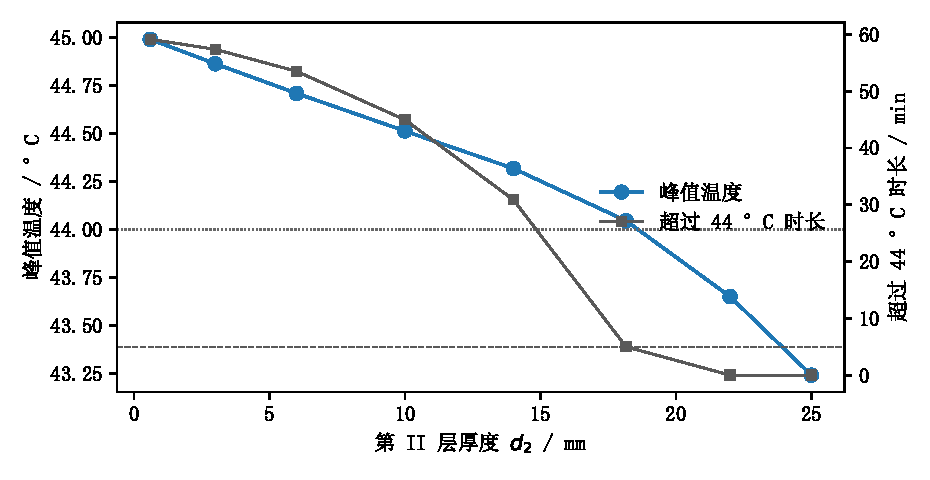
\includegraphics[width=0.86\textwidth]{figures/fig-q2-monotone.pdf}
  \caption{第 II 层厚度对峰值温度与越阈时长的影响}
  \label{fig:q2mono}
\end{figure}

二分结果为 $d_2^{*}=\SI{18.16}{mm}$。该点峰值 \SI{44.045}{\celsius}，
距 \SI{47}{\celsius} 上限还有近 \SI{3}{\celsius}，越阈时长恰为 \SI{300}{s}：
紧的是五分钟预算，不是温度上限。皮肤温度首次越过 \SI{44}{\celsius} 的时刻为
\SI{3302}{s}，即第 \SI{55.0}{min}，与前一节由单调性推出的 $T_{\mathrm{w}}-\SI{300}{s}$
一致。

\subsection{本问结果与小结}

在 \SI{65}{\celsius}、六十分钟、第 IV 层 \SI{5.5}{mm} 的条件下，第 II 层最小可行厚度为
\SI{18.16}{mm}。这一结果的可辨识性有严重限制，将在灵敏度一节单独讨论，
本问不把它当作可直接使用的设计值。

\section{问题三模型建立与求解}
\label{mcm-q2-end}
\label{mcm-q3-start}

\subsection{双目标的处理}

本问环境温度升到 \SI{80}{\celsius}，工作时长缩到 \SI{1800}{s}，$d_2$ 与 $d_4$ 同时开放，
范围分别是 $[\num{0.6},\num{25}]$ 与 $[\num{0.6},\num{6.4}]\,\si{mm}$。判据仍是
式~\eqref{eq:crit}，只把 $T_{\mathrm{w}}$ 换成 \SI{1800}{s}。

两个目标方向相反：降低成本要求 $d_2$ 小，隔热要求 $d_4$ 大。一种常见做法是把它们相减成
$\min(d_2-d_4)$。本文不采用，原因是该式隐含“第 II 层减薄 \SI{1}{mm} 与第 IV 层增厚
\SI{1}{mm} 等价”这一交换率，而题面没有给出成本与厚度的任何折算关系。两个量虽然量纲相同，
偏好含义并不相同，相减会把一个未经说明的权重写进目标函数。因此本问保留双目标：
对每个 $d_4$ 用问题二的二分求最小可行 $d_2$，报告前沿，把取舍留给有成本信息的一方。

形式上，记本问的可行集为
\begin{equation}
  \mathcal{F}=\Bigl\{(d_2,d_4):
  \max_{0\le t\le 1800}\theta(t;d_2,d_4)\le 47,\
  \bigl|\{t\le 1800:\theta(t;d_2,d_4)>44\}\bigr|\le 300,\
  d_2\in[0.6,25],\ d_4\in[0.6,6.4]\Bigr\},
  \label{eq:feas3}
\end{equation}
所报告的前沿为
\begin{equation}
  d_2^{*}(d_4)=\min\{d_2:(d_2,d_4)\in\mathcal{F}\},
  \qquad
  \mathcal{D}=\{d_4: \exists\,d_2,\ (d_2,d_4)\in\mathcal{F}\}.
  \label{eq:front3}
\end{equation}
$\mathcal{D}$ 就是下一节要给出的可行性边界；$d_2^{*}(\cdot)$ 在 $\mathcal{D}$ 上有定义，
其单调性由与问题二相同的热阻关系保证。任何一种标量化都只是在这条前沿上选一点，
因此先给前沿、再谈取舍，比先设权重更不容易把结论建立在未给条件上。

\subsection{可行性边界与前沿}

扫描 $d_4$ 时出现一条硬边界。当 $d_4\le\SI{3.6}{mm}$ 时，$d_2$ 取遍
$[\num{0.6},\num{25}]\,\si{mm}$ 都不满足式~\eqref{eq:crit}；可行性边界约在 \SI{3.8}{mm}。
这与问题一算出的稳态温降分布一致：空气层承担了总温降的六成，它薄到一定程度后，
织物层再厚也补不回来。表~\ref{tab:front} 给出可行区间内的前沿。

\begin{table}[htbp]
  \centering
  \caption{问题三前沿：每个第 IV 层厚度对应的最小可行第 II 层厚度（\SI{80}{\celsius}，三十分钟）}
  \label{tab:front}
  \begin{tabular}{cccc}
  \toprule
    $d_4$/\si{mm} & 最小可行 $d_2$/\si{mm} & 峰值/\si{\celsius} & 总厚/\si{mm} \\
  \midrule
    0.6 & 无可行解 & --- & --- \\
    1.0 & 无可行解 & --- & --- \\
    1.4 & 无可行解 & --- & --- \\
    1.8 & 无可行解 & --- & --- \\
    2.2 & 无可行解 & --- & --- \\
    2.6 & 无可行解 & --- & --- \\
    3.0 & 无可行解 & --- & --- \\
    3.4 & 无可行解 & --- & --- \\
    3.8 & 24.988 & 45.042 & 28.788 \\
    4.2 & 24.369 & 44.999 & 28.569 \\
    4.6 & 23.761 & 44.959 & 28.361 \\
    5.0 & 23.177 & 44.914 & 28.177 \\
    5.4 & 22.593 & 44.874 & 27.993 \\
    5.8 & 22.021 & 44.834 & 27.821 \\
    6.2 & 21.462 & 44.792 & 27.662 \\
  \bottomrule
\end{tabular}

\end{table}

前沿单调：第 IV 层每增厚 \SI{1}{mm}，第 II 层可减薄约 \SI{1.5}{mm}。若以总厚最小为附加偏好，
则取 $d_4=\SI{6.4}{mm}$、$d_2=\SI{21.188}{mm}$，总厚 \SI{27.588}{mm}；此时 $d_4$ 位于
附件 1 给的上界。注意前沿上每点的峰值都在 \SI{44.8}{\celsius} 到 \SI{45.0}{\celsius} 之间，
仍低于 \SI{47}{\celsius} 上限——与问题二一样，紧的是五分钟预算。

前沿的求法写清如下，它只是把问题二的一维搜索放进一层外循环。对给定的 $d_4$，
可行性判断仍由式~\eqref{eq:crit} 给出；由于固定 $d_4$ 后峰值对 $d_2$ 仍单调不增
（机理与问题二相同：加厚织物层只增加串联热阻），内层用同一段二分。外层按
\SI{0.4}{mm} 步长扫描 $d_4\in[0.6,6.4]$，共 15 个点。外层不需要二分：可行性边界
只需定位到扫描分辨率，而边界附近的 $d_2^{*}$ 已经贴近上界 \SI{25}{mm}，
再细分不会改变结论的性质。整个过程调用仿真器约 $15\times12$ 次，
在最薄层 20 格、步长 \SI{4}{s} 下可在数分钟内完成。

图~\ref{fig:q3front} 把整张表画出来。左侧阴影区是第 IV 层薄于可行性边界时的不可行带，
右侧曲线近似为直线，斜率约 $-1.5$：第 IV 层每增厚 \SI{1}{mm}，第 II 层可减薄约
\SI{1.5}{mm}。这个交换率不是题面给的，而是本模型算出来的，它正是把双目标收缩成单目标时
本应先取得的信息。

\begin{figure}[htbp]
  \centering
  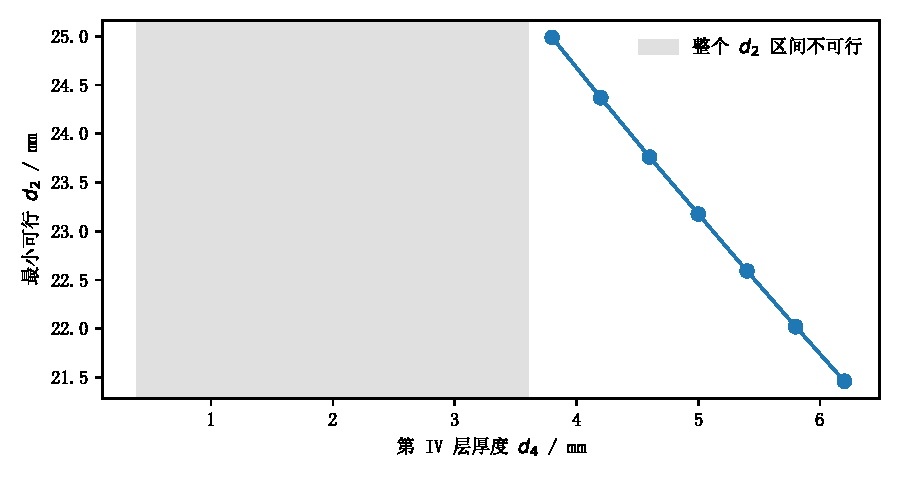
\includegraphics[width=0.84\textwidth]{figures/fig-q3-front.pdf}
  \caption{问题三前沿与不可行带}
  \label{fig:q3front}
\end{figure}

两点需要说清。第一，前沿的斜率来自热阻关系而非拟合：由表~\ref{tab:res}，
空气层的 $\lambda_4=\SI{0.028}{W/(m.K)}$ 远小于第 II 层的 $\lambda_2=\SI{0.37}{W/(m.K)}$，
单位厚度的热阻之比约为 $0.37/0.028\approx13$，因此在等热阻意义下第 IV 层增厚 \SI{1}{mm}
可以换掉第 II 层十几毫米；实际交换率只有 $1.5$，是因为可行性由越阈时刻而非总热阻决定，
瞬态过程削弱了这一比值。第二，可行性边界与题面示例的量级不符：题面在问题一中给出的
第 IV 层厚度是 \SI{5}{mm}，而问题三要求 \SI{80}{\celsius} 下工作三十分钟，
此时第 IV 层不得薄于约 \SI{3.8}{mm}，余量并不宽裕。

\subsection{本问结果与小结}

本问的可交付结论是一条前沿与一条可行性边界，而不是单点：第 IV 层不得薄于约 \SI{3.8}{mm}；
在此之上，$(d_4,d_2)$ 沿表~\ref{tab:front} 取舍。总厚最小点为 \SI{6.4}{mm} 与
\SI{21.188}{mm}。同一条可辨识性限制也适用于本问。

\section{结果分析与模型检验}
\label{mcm-q3-end}

\subsection{结果解释}

三问的结果指向同一个机理。空气层是四层里热阻最大的一层，在附件 2 的条件下单独承担
\SI{17.040}{\celsius} 的温降，占总温降的六成；它同时是扩散最快的一层，扩散时间尺度
$d^2/a$ 只有约 \SI{1}{s}。这两个性质合在一起，使空气层在稳态上决定“能挡多少”，
在瞬态上几乎不延迟“什么时候挡不住”。问题三的可行性边界就落在这里：$d_4$ 决定平台高度，
$d_2$ 只能在平台之下微调升温快慢。

问题二、三的紧约束都是五分钟预算而非 \SI{47}{\celsius} 上限，这一点值得单独说明。最优点的
平台温度只需略高于 \SI{44}{\celsius}，就能让越阈时长压到 \SI{300}{s}；而要让峰值触及
\SI{47}{\celsius}，平台需要再高近 \SI{3}{\celsius}，对应的厚度远薄于可行下限。
换句话说，题面给的两条要求中，起作用的是后一条。

最后与那份参考论文的报告值作一次对照，作为本模型的外部落点检查。把它给出的厚度直接代入
本文模型并按式~\eqref{eq:crit} 判定：$d_2=\SI{5.5}{mm}$（问题二条件）峰值
\SI{44.73}{\celsius} 未破上限，但越阈时长 \SI{3256}{s}，是预算的十倍以上；
$(d_2,d_4)=(5.6,5.4)$ 与 $(5.6,6.4)\,\si{mm}$（问题三条件）峰值分别为
\SI{48.97}{\celsius} 与 \SI{48.01}{\celsius}，直接越过 \SI{47}{\celsius} 上限。三组都不是
临界判定。需要说明的是，该文的稳态界面温度 \num{74.30}、\num{72.75}、\num{65.12}、
\SI{48.08}{\celsius} 与本文式~\eqref{eq:steady} 的结果逐项一致，其稳态代数部分是正确的。

表~\ref{tab:verdict} 把三组对照汇总。三行的失效方式并不相同：问题二那一行没有越过温度上限，
败在越阈时长——\SI{3256}{s} 是 \SI{300}{s} 预算的十倍以上；问题三两行则直接越过
\SI{47}{\celsius} 硬上限，分别高出 \SI{1.97}{\celsius} 与 \SI{1.01}{\celsius}。
两种失效对应两条不同的约束，说明不是某一条判据写法上的分歧，而是模型缺少时间维之后
两条约束都失去了控制。

\begin{table}[htbp]
  \centering
  \caption{参考论文报告厚度代入本文模型后的判定}
  \label{tab:verdict}
  \begin{tabular}{ccccc}
  \toprule
    参考论文报告值 & 峰值/\si{\celsius} & 未破 \SI{47}{\celsius} & $>\SI{44}{\celsius}$ 时长/\si{s} & 可行 \\
  \midrule
    问题二 \SI{5.5}{mm} & 44.73 & 是 & 3256 & 否 \\
    问题三 \SI{5.6}{mm}/\SI{5.4}{mm} & 48.97 & 否 & 1644 & 否 \\
    问题三 \SI{5.6}{mm}/\SI{6.4}{mm} & 48.01 & 否 & 1626 & 否 \\
  \bottomrule
\end{tabular}

\end{table}

还有一处跨问接口需要明确写出，否则读者无法判断三问的结果能否互相引用。
表~\ref{tab:iface} 列出每问冻结了什么、新开放了什么、以及输出进入了哪里。
三问共享同一个仿真器与同一个散热系数，因此问题二、三的厚度结论继承问题一的全部标定
不确定性；反过来，问题一的验证结论不因问题二、三换了环境温度而自动成立。

\begin{table}[htbp]
  \centering
  \caption{三问之间的冻结量、新开放量与输出接口}
  \label{tab:iface}
  \begin{tabular}{cllc}
    \toprule
    问 & 冻结 & 新开放 & 输出 \\
    \midrule
    一 & 附件 1 物性、附件 2 实测 & 散热系数 $h$ & $h$、温度分布 Excel \\
    二 & 仿真器、$h$、$d_4=\SI{5.5}{mm}$ & $d_2$ & $d_2^{*}$、越阈时刻 \\
    三 & 仿真器、$h$ & $d_2$、$d_4$ & 前沿 $d_2^{*}(d_4)$、可行性边界 \\
    \bottomrule
  \end{tabular}
\end{table}

\subsection{模型检验}

检验分四层，每层针对一个不同的主张。

内部正确性。把环境温度固定并推进到足够长，瞬态解应收敛到式~\eqref{eq:steady} 的解析稳态解。
实际结果为 \num{47.934716682627} 与 \SI{47.934716682526}{\celsius}，相差
\SI{1e-10}{\celsius}。这同时检查了三对角组装、Robin 边界并入和式~\eqref{eq:face} 的面温还原。

离散无关性。把每层格数由 10 加密到 80、时间步长由 \SI{4}{s} 缩到 \SI{1}{s}，
共 12 组组合，终点温度相互最大偏差 \SI{2.7e-9}{\celsius}，总格数覆盖 253 到 2027。
式~\eqref{eq:harmonic} 的调和平均使界面处不引入额外离散误差，这是偏差如此之小的原因。

量纲与参数对账。逐层按 $a_i=\lambda_i/(\rho_i c_i)$ 计算得
\SI{1.985e-7}{}、\SI{2.044e-7}{}、\SI{3.514e-7}{}、\SI{2.361e-5}{m^2/s}，
与附件 1 预置的扩散系数列逐位一致，含空气层。这一步是专门设置的：如前所述，
把 $\lambda$ 误当作 $a$ 会让显式格式反而稳定，错误不会由程序报错暴露。

预测证据。用最小二乘标定的 $h$ 对附件 2 全程作预测，残差均方根 \SI{0.4517}{\celsius}，
最大绝对偏差 \SI{1.7972}{\celsius}。分段看，末三十分钟为 \SI{0.1453}{\celsius}，
前十分钟为 \SI{1.2798}{\celsius}。残差集中在升温初段，这与假设三直接相关：
第 I 层外表面并不真的瞬间达到环境温度，实际升温有一个过程。本文没有修正该假设，
因此如实报告这一段的代价：模型在平台附近可靠，在最初十分钟内偏乐观。
由于问题二、三的判据由平台附近的越阈时刻决定，该偏差不改变本文结论的方向，
但它是最先应该被改进的地方。

表~\ref{tab:resid} 把残差按时段拆开，可以看清偏差的结构而不只是一个总量。

\begin{table}[htbp]
  \centering
  \caption{模型与附件 2 的残差按时段分解}
  \label{tab:resid}
  \begin{tabular}{ccccc}
  \toprule
    时段/\si{min} & 样本数 & 残差均方根/\si{\celsius} & 最大绝对偏差/\si{\celsius} & 平均偏差/\si{\celsius} \\
  \midrule
    0--10 & 600 & 1.2798 & 1.7972 & +1.1767 \\
    10--21 & 660 & 0.2260 & 0.5933 & +0.1178 \\
    21--40 & 1140 & 0.1388 & 0.1455 & -0.1383 \\
    40--60 & 1200 & 0.1453 & 0.1453 & -0.1453 \\
    60--90 & 1801 & 0.1453 & 0.1453 & -0.1453 \\
  \bottomrule
\end{tabular}

\end{table}

三点值得读出来。第一，偏差不是随机噪声：前十分钟的平均偏差为
$+\SI{1.1767}{\celsius}$，符号一致，说明模型系统性地升温过快，这与“外表面瞬间达到
环境温度”的假设方向吻合。第二，进入准稳态后偏差迅速消失，第 \SI{21}{min} 之后各段
残差均方根都在 \SI{0.25}{\celsius} 以内，最后三十分钟只有 \SI{0.1453}{\celsius}；
这说明稳态部分的热阻链和散热系数是可靠的。第三，最大绝对偏差
\SI{1.7972}{\celsius} 出现在前十分钟内，而不在末段，因此它不影响以平台为判据的结论。

至此四层验证的对象、证据与结论可以并列写出：内部正确性以解析稳态解为参照，
离散无关性以 12 组网格步长组合为证据，量纲与参数以附件 1 的预置列为对账基准，
预测能力以附件 2 的分段残差为证据。四层各自针对一个不同的主张，
其中没有任何一层能替代另一层——例如离散无关性再好也不说明散热系数标定正确，
残差再小也不说明模型能外推到别的环境温度。

\section{灵敏度与稳健性分析}

全模型只有 $h$ 一个自由参数，因此稳健性问题集中在它上面。表~\ref{tab:sens} 给出扰动 $h$ 时
问题二最优厚度的变化。

\begin{table}[htbp]
  \centering
  \caption{问题二最优厚度对散热系数的敏感性，并列出对应的平台温度}
  \label{tab:sens}
  \begin{tabular}{ccccc}
  \toprule
    $h$ 偏移 & $h$/\si{W/(m^2.K)} & 平台温度/\si{\celsius} & 与 \SI{44}{\celsius} 之差 & 最小可行 $d_2$/\si{mm} \\
  \midrule
    -20\% & 7.0192 & 45.3929 & +1.3929 & 整区间不可行 \\
    -10\% & 7.8965 & 44.7174 & +0.7174 & 22.47 \\
    -5\% & 8.3352 & 44.4188 & +0.4188 & 20.52 \\
    -2\% & 8.5985 & 44.2505 & +0.2505 & 19.19 \\
    +0\% & 8.7739 & 44.1425 & +0.1425 & 18.18 \\
    +2\% & 8.9494 & 44.0376 & +0.0376 & 17.04 \\
    +5\% & 9.2126 & 43.8860 & -0.1140 & 14.90 \\
    +10\% & 9.6513 & 43.6473 & -0.3527 & 10.04 \\
    +20\% & 10.5287 & 43.2164 & -0.7836 & 0.60 \\
  \bottomrule
\end{tabular}

\end{table}

结果必须直说：仅 \SI{2}{\percent} 的偏移——也就是本文两条标定路线之间的差距——就使最优厚度
在 \SI{17.04}{mm} 与 \SI{19.19}{mm} 之间移动；\SI{20}{\percent} 时可行域从整体不可行跳到
下界即可行，跨越整个允许区间。

图~\ref{fig:q2sens} 把这一关系画出来，阴影带是两条标定路线之间的 \SI{2}{\percent} 精度带。
曲线在带内已经跨越约 \SI{2}{mm}，向右继续下探到下界：可辨识性问题不是由极端扰动
制造出来的，在标定自身精度内就已存在。

\begin{figure}[htbp]
  \centering
  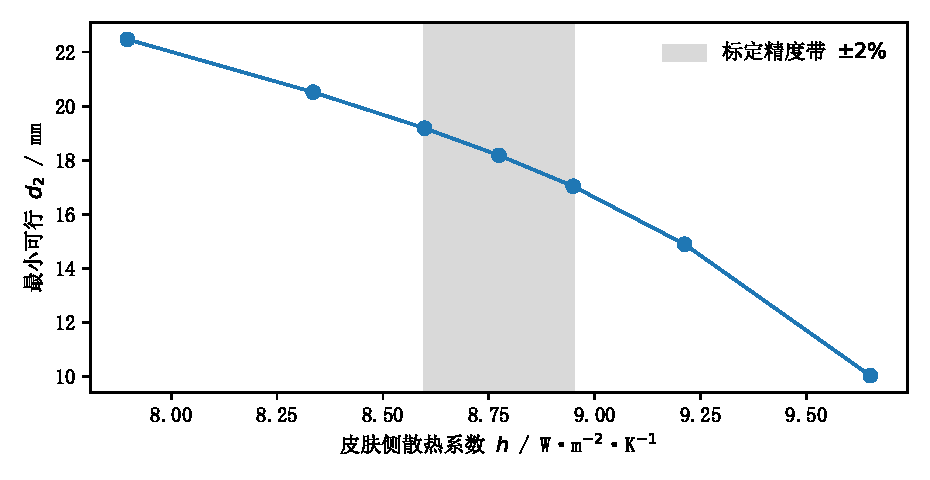
\includegraphics[width=0.86\textwidth]{figures/fig-q2-sensitivity.pdf}
  \caption{问题二最小可行厚度对皮肤侧散热系数的依赖}
  \label{fig:q2sens}
\end{figure}

机理可以定量说清。最优解必然把平台温度贴在阈值上：$d_2^{*}$ 处平台为
\SI{44.1425}{\celsius}，只比 \SI{44}{\celsius} 高 \SI{0.1425}{\celsius}。而皮肤温度曲线在
后半段已经很平，斜率由第 \SI{10}{min} 的 \SI{0.3405}{\celsius\per\minute} 降到第
\SI{55}{min} 的 \SI{0.0112}{\celsius\per\minute}。$h$ 变动 \SI{10}{\percent} 时平台在
\SI{44.7174}{\celsius} 与 \SI{43.6473}{\celsius} 之间移动，越过或退到阈值另一侧；
在近乎水平的曲线上，平台移动零点几度就把越阈时刻推移数分钟，进而要求厚度大幅改变。

表~\ref{tab:slope} 给出最优点处皮肤温度曲线的逐段斜率。第 \SI{5}{min} 时曲线还在以
每分钟半度以上的速度上升，到第 \SI{55}{min} 只剩 \SI{0.0112}{\celsius\per\minute}，
相差近两个量级。约束要求的穿越时刻恰好落在最平的那一段，这是病态性的直接来源：
若阈值定在升温初段（例如要求不得在第 \SI{5}{min} 前越过某温度），同样的参数扰动
只会引起很小的厚度变化。

\begin{table}[htbp]
  \centering
  \caption{最优点处皮肤外侧温度的逐段斜率（\SI{65}{\celsius}，$d_2=\SI{18.16}{mm}$）}
  \label{tab:slope}
  \begin{tabular}{ccc}
  \toprule
    时刻/\si{min} & 皮肤外侧温度/\si{\celsius} & 斜率/(\si{\celsius\per\minute}) \\
  \midrule
    5 & 37.8923 & +0.3740 \\
    10 & 39.7742 & +0.3405 \\
    20 & 42.0998 & +0.1616 \\
    30 & 43.1887 & +0.0755 \\
    40 & 43.6972 & +0.0352 \\
    50 & 43.9346 & +0.0165 \\
    55 & 44.0004 & +0.0112 \\
    60 & 44.0454 & +0.0077 \\
  \bottomrule
\end{tabular}

\end{table}

表~\ref{tab:sens} 的第三、四列把这件事说得更直接：$h$ 每变动 \SI{2}{\percent}，
平台温度改变约 \SI{0.11}{\celsius}，而平台与阈值之差本身只有 \SI{0.1425}{\celsius}。
也就是说，标定精度与判据余量是同一量级——这不是模型不够精细，
而是这道约束在这组条件下本身没有留出可辨识的余量。

因此“六十分钟内超过 \SI{44}{\celsius} 不超过五分钟”这一约束在本题是病态条件：
它的解位于曲线几乎水平的区段，对唯一标定参数极度敏感。本文的交付物相应地是区间与机理，
而不是三位有效数字的厚度。在标定自身精度内，问题二的可辨识区间约为 \SI{17}{mm} 到
\SI{19}{mm}。

需要区分两件事。上述病态性针对本文自己的最优厚度；对参考论文报告值的判定不受影响，
因为那三组值分别超预算十倍以上或越上限近 \SI{2}{\celsius}，远离任何边界。

要把区间收窄到工程可用精度，缺的不是算法而是数据：$h$ 只由一次 \SI{75}{\celsius} 实验定出，
它在 \SI{65}{\celsius} 与 \SI{80}{\celsius} 下是否仍取同值没有证据，而血流灌注本身随热负荷
变化。至少需要第二个环境温度下的实测曲线，或对皮肤侧散热的独立测量。

\section{模型评价与改进}

\subsection{模型评价}

本文的做法是让一个计算核心服务三问：问题一在这个核心上标定唯一参数并接受实测检验，
问题二、三冻结它只新开放厚度。这样做的好处不只是省事，而是让题面里的时间量始终有表达位置；
一旦某一问换成无时间维的代数式，六十分钟、三十分钟和五分钟就无处安放。
界面导度取调和平均使热流连续在离散层面精确成立，这是终点温度对网格几乎不敏感的原因。

表~\ref{tab:sum} 汇总三问的条件、结论与紧约束。三问的紧约束都是五分钟预算，
这本身是一个可以核对的结论：它意味着若把题面的 \SI{47}{\celsius} 上限改成
\SI{46}{\celsius} 或 \SI{48}{\celsius}，本文的厚度结果都不会改变；
真正敏感的是 \SI{44}{\celsius} 这条阈值和五分钟这个预算。

\begin{table}[htbp]
  \centering
  \caption{三问结论汇总}
  \label{tab:sum}
  \begin{tabular}{clll}
  \toprule
    问 & 条件 & 结论 & 紧约束 \\
  \midrule
    一 & \SI{75}{\celsius}，\SI{90}{min} & $h=\SI{8.7739}{W/(m^2.K)}$，温度分布 & 无（标定问） \\
    二 & \SI{65}{\celsius}，\SI{60}{min} & $d_2^{*}=\SI{18.16}{mm}$ & 五分钟预算 \\
    三 & \SI{80}{\celsius}，\SI{30}{min} & 前沿 $d_4\ge\SI{3.8}{mm}$，总厚最小 \SI{27.588}{mm} & 五分钟预算 \\
  \bottomrule
\end{tabular}

\end{table}

三处局限已在正文中定量报告：升温前十分钟残差 \SI{1.2798}{\celsius} 反映外侧边界假设过强；
$h$ 的跨环境温度可迁移性没有证据；问题二的解在标定精度内只能定到约 \SI{2}{mm} 的区间。
其中第三条不是数值方法的问题，而是约束本身的条件数决定的。

不考虑湿传递是本文最大的结构性简化。在高温高湿的实际作业中，汗液蒸发与水汽迁移会显著改变
有效热阻，其影响很可能超过上面报告的参数敏感性。附件没有给出可用于标定这一机制的任何量，
因此本文没有把它写进方程，而不是认为它可以忽略。

\subsection{改进方向}

按可执行性排序。第一，把外侧边界从 Dirichlet 改成带表面传热系数的 Robin 型，
使第 I 层表面温度有一个上升过程，这可直接改善前十分钟的残差，代价是多一个待定参数，
需要用残差前段单独标定。第二，在第二个环境温度下补一次假人实验，用两条曲线联合标定 $h$，
或直接检验它是否随环境温度变化；这是把问题二区间收窄的唯一可靠途径。第三，若能获得
成本与厚度的折算关系，问题三的前沿即可收缩为单点，此时相减型标量化才有依据。
第四，引入湿传递需要新的实验设计，不属于当前数据能支持的改进。

\label{mcm-body-end}
\section{参考文献}

本文的数值结论只依赖官方附件 1、附件 2 与本文自编程序，未引用外部文献结果。
正文中与参考论文的对照仅用于说明本模型在同一组厚度下的判定，其数据来源已在相应位置注明。

\section{附录：代码、数据与补充结果}

\subsection{程序与文件清单}

\begin{table}[htbp]
  \centering
  \caption{支撑材料清单}
  \label{tab:materials}
  \begin{tabular}{lll}
    \toprule
    文件 & 作用 & 说明 \\
    \midrule
    \texttt{solver/simulator.py} & 仿真器与三问求解 & 含标定、收敛检查、二分与前沿扫描 \\
    \texttt{inputs/attachment.xlsx} & 官方附件 1、附件 2 & 未修改 \\
    \texttt{results/run-report.json} & 一次运行的全部数值 & 标定、验证、收敛、问二问三 \\
    \texttt{results/conclusions.json} & 结论与可辨识性限制 & 含敏感性表与机理 \\
    \bottomrule
  \end{tabular}
\end{table}

\subsection{支撑材料文件清单与运行说明}

全部数值由一条命令产生：

\begin{verbatim}
python solver/simulator.py --self-test
\end{verbatim}

该命令读取 \texttt{inputs/attachment.xlsx}，完成两条路线标定、附件 2 残差评估、
网格与步长收敛检查、问题二二分与问题三前沿扫描，并把结果写入
\texttt{results/run-report.json}。正文所有数值均可在该文件中按字段定位，
不存在正文与程序输出不同源的情形。

\subsection{完整可运行源程序与附件说明}

源程序见 \texttt{solver/simulator.py}。主要接口为：\texttt{read\_materials} 与
\texttt{read\_measurement} 读取附件；\texttt{Simulator} 按层分配格心网格并按
式~\eqref{eq:harmonic} 组装界面导度，\texttt{run} 按式~\eqref{eq:implicit} 逐步推进并按
式~\eqref{eq:face} 还原面温；\texttt{calibrate\_skin\_coefficient} 给出两条标定路线；
\texttt{constraint\_metrics} 按式~\eqref{eq:crit} 逐时刻判定；
\texttt{minimal\_feasible\_d2} 在已确认的单调性上做二分；\texttt{pareto\_d2\_d4} 生成
问题三前沿。

\end{document}







